%!TEX root=./paper.tex
\section{System Model}\label{sec:system-model}
\subsection{\textbf{Data streaming framework}}

Reliable real-time data collection is a crucial aspect and prerequisite of a digital twin to effectively update internal parameters and synchronize with the real world. The Traffic Digital Twin (TDT), \name, presented in this paper requires real-time traffic volume data as input. We aim to use absolute traffic volume counts available at a manageable low frequency of 15 minutes to one hour. While systems with more sophisticated data at a higher frequency can be proposed, we aim to keep the real-world collection infrastructure cheap, simple, and based on already existing systems around the world. In particular, we strive to cater to the following objectives:

\begin{figure*}[t]
  \centering
  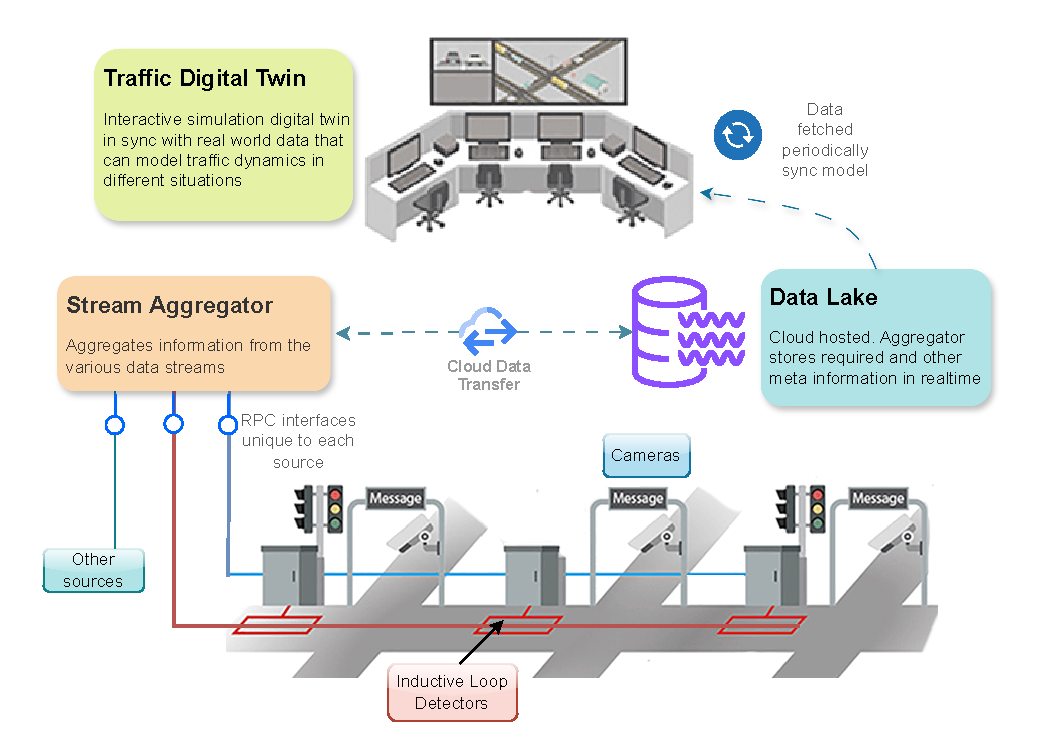
\includegraphics[width=0.77\textwidth]{framework.pdf} % Adjust width as needed
  \caption{Traffic Digital Twin (TDT) data processing}
  \label{fig:framework}
\end{figure*}

\begin{enumerate}[(i)]
    \item Hardware infrastructure should be cheap and easily replaceable.
    \item Easily extendable to use a variety of different sources.
    \item Should work with only absolute traffic counts, no other specific information like direction and vehicle types.
    \item Should work with a medium-frequency update.
\end{enumerate}

There are various possible ways to collect the type of data mentioned. The most reliable would be to install inductive loop detectors embedded in road surfaces at city intersections. Such systems are already available and in use in several major cities. For example, the Sydney Coordinated Adaptive Traffic System (SCATS)\cite{scats} is available in over 180 cities across 28 countries, including New Zealand, Dublin, Shanghai, and Hong Kong \cite{wiki:sydney_traffic_system}. New York City's Adaptive Traffic Control System (ATCS), Adaptive Signal Control Technology (ASCT), SCOOT, and ACS are other such systems that are used to control traffic signal timings and optimize congestion. Such systems can be easily extended to use with our proposed model since we only use absolute traffic volume counts, which such systems are capable of collecting.

Another possible data source can be surveillance cameras assisted with computer vision models\cite{jain2019review}, which is already used in practice at some intersections in Shenzhen, China. Several existing studies\cite{asha2018vehicle} using state-of-the-art object detection models like YOLO\cite{redmon2018yolov3} demonstrate the effectiveness of this method. Such a model-based approach allows for cheap and effective traffic monitoring on top of existing surveillance camera infrastructure. 

Other methods like using GPS-enabled mobile phones\cite{rose2006mobile} to track urban traffic flow, as Google does in its Maps product, and the use of probe vehicles\cite{zhu2012probe}, which are vehicles equipped with detectors that may be taxis or public transport, can also be used to approximate traffic volume based on their data.

We aim for our model to work in conjunction with multiple data streams, as different parts of the road network may be served with different data sources. We want our TDT to integrate with these sources seamlessly, so we need an aggregator of sorts to reconcile the data from the different streams and store them in a data lake. This data can then be used by the TDT model to keep its internal state in sync with real-world data.

The deployed aggregator system will have an RPC and API interface that can be interacted with by the remote sensors and other data sources. Each service can have a separate interface built for interacting with the aggregator service. The aggregator then stores all the data with relevant meta information in a datalake, a centralized repository that allows you to store all your structured and unstructured data. We make use of a datalake as different sources might have additional information apart from just traffic volume counts, and by allowing us to store other complementary information, we leave possible avenues for building up further capabilities in our TDT.

An example representing a simplified view of the aforementioned process is shown in Fig. \ref{fig:framework}.